
Das WebGL Koordinaten System
Aufbau der Oberfl�che
Grunds�tzliches zur Navigation im 3D Raum



SumoViz3D verwendet eine perspektivische Kamera mit einem festeingestellten Sichtfeld von $45^\circ$. Die Positionierung und Ausrichtung der Kamera ist, mit einigen Einschr�nkungen, dem Nutzer �berlassen. W�hrend der Visualisierung kann Kameraposition und -ausrichtung ver�ndert werden. Dazu wurde die Klasse \verb+SphereControls+ angelegt. Im Konstruktor der Klasse wird das Kamera-Objekt �bergeben, dessen Position manipuliert werden soll und das DOM-Element auf dem die Benutzereingaben erfolgen, in diesem Fall also das canvas-Element. Damit werden nur Eingaben die direkt auf dem canvas-Element erfolgen verarbeitet. Eingaben auf den HTML-Overlay-Elementen wie der Toolbar oder Dialogen werden f�r die Kamerasteuerung ignoriert. Event-Listener die auf Tastatur- und Mouseeingaben reagieren werden mittels \verb+addEventListener+ an das canvas-Element angef�gt.

\begin{wrapfigure}{l}{0.5\textwidth}
  \begin{center}
    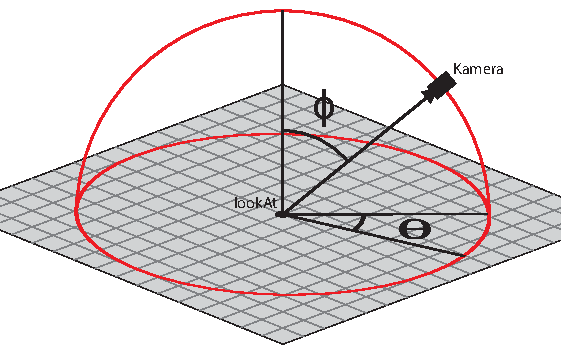
\includegraphics[width=0.5\textwidth]{media/camera.pdf}
  \end{center}
  \caption{A gull}
  \label{cameramodel}
\end{wrapfigure}




Zur Ausrichtung der Kamera wird der Punkt \verb+lookAt+ definiert, auf den die Kamera stets ausgerichtet ist. Dieser Punkt liegt immer in der Grundebene der dargestellten Geometrie und kann dort bewegt werden. Die Kamera kann sich halbkugelf�rmig um diesen Punkt herum bewegen und dabei nicht unterhalb der Grundebene bewegt werden. Zur Berechnung der Position der Kamera sind neben der Position des \verb+lookAt+-Punktes noch der Radius $r$ der Kugel, der Neigungswinkel $\theta$ und der Drehwinkel $\phi$ notwendig. Mit folgenden Formeln lassen sich die Positionskoordinaten wie folgt berechnen:
\begin{eqnarray*}x = lookAt.x + r \cdot \sin \theta \cdot \cos \phi \\
y = lookAt.z + r \cdot \cos \theta
z = lookAt.y + r \cdot \sin \theta \cdot \sin \phi \qquad (0 \le \theta \le \pi \ \wedge 0 \le \phi < 2 \pi) \\
\end{eqnarray*}



\begin{tabular}{lll}
\textbf{EventListener} & \textbf{} &\textbf{Funktionalit�t} \\
\hline
\verb+keydown+                     & \verb+lookAt+ & Bewegen  \\
\verb+mousedown+ + \verb+mousemove+       & $\theta$ und $\phi$ & Kamera drehen und neigen \\
\verb+mousewheel+ (\verb+DOMMouseScroll+\footnotemark) & $r$ & Zoomen \\
\verb+contextmenu+              &   \multicolumn{2}{l}{Objekte anpassen}  \\

\end{tabular}

\footnotetext{In Firefox verwendet}



In der Animations-Schleife wird die \verb+update+-Methode der Steuerung aufgerufen. Ist ein \verb+keydown+- aber noch kein \verb+keyup+-Event auf einer der Cursor-Tasten ausgel�st, so ist diese Cursor-Taste gerade gedr�ckt und die Position des \verb+lookAt+-Punkts wird in entsprechender Richtung ver�ndert....


F�r das Drehen und Neigen der Kamera wird die Distanz zwischen dem Punkt, an dem das \verb+mousedown+-Event ausgel�st wurde und der aktuellen Mousecursorposition berechnet. Die horizontale Distanz wird auf den Drehwinkel $\phi$ addiert und bewegt die Kamera im mathematischen Drehsinn auf der Kugeloberfl�che. Wird die Mouse nach links gezogen, so hat die Distanz einen negativen Wert und wird vom Drehwinkel subtrahiert, was eine Bewegung gegen den mathematischen Drehsinn zur Folge hat. Die vertikale Distanz wird vom Neigungswinkel $\theta$ subtrahiert, da dieser der Y-Achse her aufgespannt wird (vgl. Abbildung \ref{cameramodel}). Au�erdem wird verhindert das $\theta > \frac{\pi}{2}$, um stets �ber der Grundebene zu bleiben.